
% We aim to improve the robustness of BERT~\citep{devlin2018bert} when trained to solve a natural language inference task. Hereafter, we describe the dataset used for this task as well present our methodology.

\subsection{Datasets: MNLI and HANS}
\label{sec:dataset}
The MNLI corpus~\citep{williams2017broad} is a popular NLU dataset containing premise/hypothesis pairs annotated with textual entailment information (neutral, entailment or contradiction). Multiple studies have hypothesized that deep learning models tend to capture simple heuristics from the MNLI training data, and do not build an actual understanding of the task. Over the years, a series of diagnostic datasets have been released to test these hypotheses.
The very recent of these datasets, HANS~\citep[Heuristic Analysis for NLI Systems]{linzen2019right}, contains curated templates designed to test the robustness of a model against the following three heuristics for recognizing if a premise entails a hypothesis: lexical overlap (a premise entails any hypothesis built from of a subset of its words), subsequence (a premise entails any of its contiguous subsequences) and constituent (a premise entails all the complete subtrees in its parse tree). In particular, any model relying exclusively on those heuristics would not have a higher than chance classification accuracy on this test set.

\citet{linzen2019right} show that a variety of existing models -- including BERT~\citep{devlin2018bert}, the state-of-the-art model at the time -- perform, overall, worse than chance on classification accuracy of HANS evaluation data. This confirms the hypothesis that models trained on MNLI data tend to learn the three aforementioned heuristics rather than actually understanding the task. To test our methodology, we thus make use of the HANS evaluation dataset, which contains 30,000 examples equally split between the two labels: ``entailment'' and ``non-entailment''.

\subsection{Weak Baselines}
% as: here you need to restress that the weak baselines will serve as "bias models", i.e. we hope they will capture biases in the dataset and forgettable example will correspond to those example that do not match the biases (contribution of the paper basically)

We train two models, BoW and BiLSTM, as our weak baselines to compute forgetting statistics of different examples in the training set. We use the term weak to emphasize the fact that those models have fewer parameters than our base model BERT (we default to the ``base'' configuration of the BERT model). Our conjecture is that networks with lower capacity will discover the samples that support the various heuristics described in Section \ref{sec:dataset}. In particular, \emph{forgettable} examples for those models will correspond to sentences that do not verify said heuristics.

Both models are siamese networks, with similar input representations and classification layers.
For the input layer, we lower case and tokenize the inputs into words and initialize their representations with Glove, a 300 dimensional pretrained embedding~\citep{pennington2014glove}.
For the classification task, from the premise and hypothesis vectors $p$ and $h$, we build the concatenated vector $s = [p, h, |p - h|, p \odot h]$ and pass it to a two-layer perceptron classifier. 
To compute $p$ or $h$, the BoW model max-pools the bag of word embeddings,
while the BiLSTM model max-pools the top-layer hidden states of a 2-layer bidirectional LSTM. The hidden size of the LSTMs is set to 200.

\begin{table}[t]
\footnotesize
\caption{Number of ``forgettables'' examples (those that are forgotten at least once or never learned) during five training epochs along with the accuracy on the MNLI matched development set.}
\label{tab:forg_stats}
\centering
\begin{tabular}{lccc}
\toprule
Model & \# Forg. & \# Forg. (balanced) & MNLI\\
\midrule
BoW         &100,345 & \balancedbow & 64.0\\
BiLSTM      &76,270 & \balancedlstm  & 69.6\\
% BiLSTM-ATT  & 76,903 & 70.5\\
BERT        &32,387 &  \balancedbert & 84.5\\
\bottomrule
\end{tabular}
\end{table}

\subsection{Computing forgetting events}
\label{sec:forg_stat}
For each of the three models (i.e., the two weak baselines and BERT) we train on all MNLI training examples for five epochs and calculate the number of times each example is forgotten, following the same procedure described in \citet{toneva2018empirical}. In short, an example is forgotten if it goes from being correctly to incorrectly classified (because of multiple gradient updates performed on other examples).

If an example is forgotten at least once or is never learnt during training, we call it ``forgettable''. %TODO keep forgettable term consistent 
In Table \ref{tab:forg_stats}, the numbers of forgettable examples for BoW, BiLSTM and BERT models are shown. 
To remove the effect of bias in label distribution, we sample forgettable examples for each label to keep the label distribution the same as the original MNLI training data (i.e., 33\% from each of the three label). The size of the balanced forgettables for each model is also shown in Table \ref{tab:forg_stats}.
We make use of the balanced forgettable sets in Section \ref{sec:eval}.
It is worth noting that the larger the model, the fewer the forgettable examples. We also include the performance of the models on the development set of MNLI.
Figure~\ref{fig:trainingsize-unsup} shows the distribution of forgetting events.

\begin{figure}[t]
\centering
  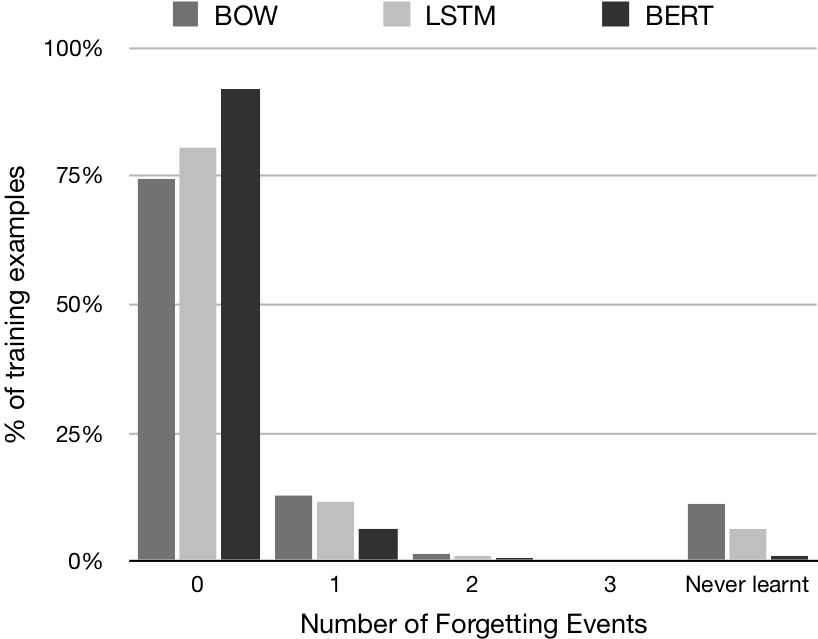
\includegraphics[width=0.45\textwidth]{figures/bar_chart.png}
  \caption{Distribution of forgetting events for the three models after five training epochs. As can be seen, a majority of examples are not forgotten during training. We make use of examples 
  with at least one forgetting event in our method for robust NLI models.}
%   \caption{The percentage of training examples for each number of forgetting count after five training epochs. 
%   The examples with 5 forgetting count
%   are the unlearned ones.} 
\label{fig:trainingsize-unsup}
\end{figure}


\subsection{Fine-tuning on forgettable examples}
We adopt a simple strategy to exploit the sets of forgettables computed by one of our baselines or BERT itself: we first fine-tune BERT on all the MNLI examples in order to get a reasonable prior for the task. We then perform an additional stage of fine-tuning ($3$ epochs) only on the subset of selected forgettable examples from each of the considered models.

\iffalse
\subsection{Comparing our methodology to related work}
\begin{itemize}
    \item The recent work to tackle the brittleness of MNLI trained models all are built based on the prior knowledge about the biases
    in the training dataset. 
    
    
    Notably, \newcite{clark2019dont} introduce a 2 stage process as:
\begin{quote}
        (1)
train a naive model that makes predictions exclusively based on dataset biases, and (2) train
a robust model as part of an ensemble with the
naive one in order to encourage it to focus on
other patterns in the data that are more likely to
generalize
    \end{quote}
    
    \newcite{he2019unlearn} employs a similar approach and uses a bag-of-word, a hypotheis-only and a manually-built bias models, and fits 
    their target model to the residual of these weak baselines.
    
    \newcite{mahabadi2019simple} takes a very similar approach as in \newcite{clark2019dont}.
    
    In compared to these methods, we do not rely on known biases and prior knowledge about the dataset.
    We do however rely on weaker models to compute a more diverse set of forgettables.

\end{itemize}
\fi